\section{Neural Geometry Fields (NGFs)}\label{Sec:MainPart}

Sivaram and colleagues divide the Neural Geometry Fields pipeline into three distinct stages.

First, they input a base mesh \( \Sigma \) and partition it into quadrangular patches.
From this, they construct a trainable feature field \( \Psi : \Sigma \to \mathbb{R}^F \), associating each patch with a set of features that describe its surface properties, where each feature consists of \( F \) real components.
In the second stage, they feed these features, along with the 3D positions of the mesh, into a neural network that computes the displacement for each point on the mesh.
They then apply the displacements to the base mesh, producing a transformed conventional triangle mesh.
Finally, they optimize the feature field and patches using an inverse rendering algorithm.

In the following sections, we explore each stage in greater detail and provide an example to clarify the process further.






\subsection{Surface Partitioning into Patches}

Sivaram and colleagues introduce a method for surface representation by partitioning a simplified base mesh, denoted as $\Sigma$, into quadrilateral patches $\sigma$.
To achieve this, they greedily merge adjacent triangles into near-rectangular quads.
This process serves as a simplification step that reduces the meshs topological complexity, eliminates non-manifold configurations and results in a more compact and regular representation of the surface geometry.
By relying on quadrilateral patches rather than a purely triangular mesh, they decrease the overall number of patches and simplify the interpolation domain for later processing.
\usetikzlibrary{calc, shapes.geometric, arrows.meta, decorations.pathreplacing, positioning, shapes}
\begin{figure}[ht]
  \centering
  \begin{adjustbox}{center}
  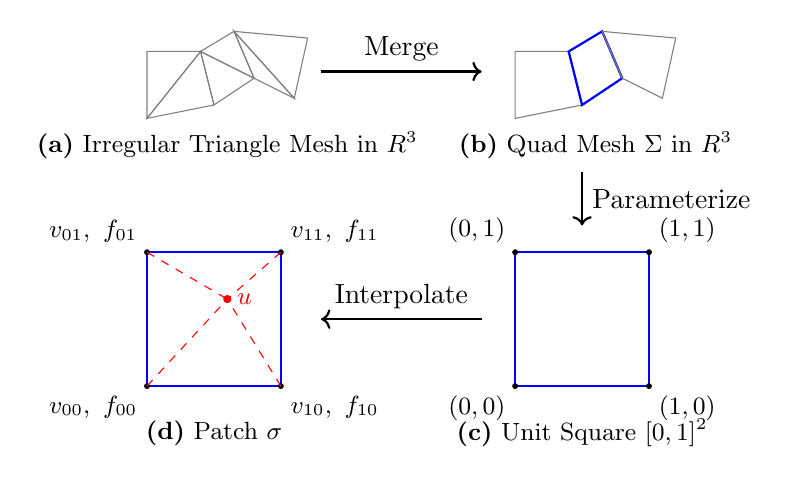
\begin{tikzpicture}[scale=0.85]

    % === Triangle Mesh (Left) ===
    \begin{scope}
      \coordinate (A) at (0,0);
      \coordinate (B) at (1,0.2);
      \coordinate (C) at (0.8,1);
      \coordinate (D) at (0,1);
      \coordinate (E) at (1.6,0.6);
      \coordinate (F) at (1.3,1.3);
      \coordinate (G) at (2.2,0.3);
      \coordinate (H) at (2.4,1.2);

      \draw[gray] (A) -- (B) -- (C) -- cycle;
      \draw[gray] (A) -- (C) -- (D) -- cycle;
      \draw[gray] (B) -- (E) -- (C) -- cycle;
      \draw[gray] (C) -- (E) -- (F) -- cycle;
      \draw[gray] (E) -- (G) -- (F) -- cycle;
      \draw[gray] (F) -- (G) -- (H) -- cycle;
      \node at (1.2, -0.4) {\small \textbf{(a)} Irregular Triangle Mesh in $\mathbb{R}^3$};
    \end{scope}

    % === Merge Arrow ===
    \draw[->, thick] (2.6,0.7) -- (5.0,0.7) node[midway, above] {Merge};

    % === Quadrilateral Mesh (Middle) ===
    \begin{scope}[xshift=5.5cm]
      \coordinate (A) at (0,0);
      \coordinate (B) at (1,0.2);
      \coordinate (C) at (0.8,1);
      \coordinate (D) at (0,1);
      \coordinate (E) at (1.6,0.6);
      \coordinate (F) at (1.3,1.3);
      \coordinate (G) at (2.2,0.3);
      \coordinate (H) at (2.4,1.2);

      \draw[gray] (A) -- (B) -- (C) -- (D) -- cycle;
      \draw[blue, thick] (B) -- (E) -- (F) -- (C) -- cycle; % highlighted patch
      \draw[gray] (E) -- (G) -- (H) -- (F) -- cycle;

      \node at (1.2, -0.4) {\small \textbf{(b)} Quad Mesh $\Sigma$ in $\mathbb{R}^3$};
    \end{scope}

    % === Down Arrow to Unit Square ===
    \draw[->, thick] (6.5,-0.8) -- (6.5,-1.6) node[midway, right] {Parameterize};

    % === Unit Square (Right) ===
    \begin{scope}[xshift=5.5cm, yshift=-4.0cm]
      \draw[blue, thick] (0,0) rectangle (2,2);
      \filldraw[black] (0,0) circle (1pt) node[anchor=north east] {\small $(0,0)$};
      \filldraw[black] (2,0) circle (1pt) node[anchor=north west] {\small $(1,0)$};
      \filldraw[black] (0,2) circle (1pt) node[anchor=south east] {\small $(0,1)$};
      \filldraw[black] (2,2) circle (1pt) node[anchor=south west] {\small $(1,1)$};
      \node at (1,-0.7) {\small \textbf{(c)} Unit Square $[0,1]^2$};
    \end{scope}

    % === Left Arrow to Feature Field ===
    \draw[->, thick] (5.0,-3) -- (2.6,-3) node[midway, above] {Interpolate};

    % === Feature Field (Left) ===
    \begin{scope}[yshift=-4.0cm]
      \draw[blue, thick] (0,0) rectangle (2,2);

      % Corner features (bold vectors), with f00 label moved outward
      \filldraw[black] (0,0) circle (1pt) node[anchor=north east] {\small $\bm{v_{00}},\ \bm{f_{00}}$};
      \filldraw[black] (2,0) circle (1pt) node[anchor=north west] {\small $\bm{v_{10}},\ \bm{f_{10}}$};
      \filldraw[black] (0,2) circle (1pt) node[anchor=south east] {\small $\bm{v_{01}},\ \bm{f_{01}}$};
      \filldraw[black] (2,2) circle (1pt) node[anchor=south west] {\small $\bm{v_{11}},\ \bm{f_{11}}$};

      % Interpolation point (u)
      \filldraw[red] (1.2,1.3) circle (1.5pt) node[right] {\small $\bm{u}$};

      % Lines from corners to interpolation point
      \foreach \x/\y in {0/0, 2/0, 0/2, 2/2} {
        \draw[dashed, red] (\x,\y) -- (1.2,1.3);
      }

      % Patch label
      \node at (1,-0.7) {\small \textbf{(d)} Patch $\sigma$};
    \end{scope}
    
  \end{tikzpicture}
  \end{adjustbox}
  \caption{Surface processing pipeline: The irregular triangle mesh is simplified and merged into a quadrilateral mesh $\Sigma$. A quadrilateral patch is extracted, which is then parameterized over the unit square $[0,1]^2$. This parameterization facilitates both geometric and feature field interpolation, with feature values interpolated at the patch's corners and at an arbitrary point $\bm{u}$. Inspired by~\cite{sivaram2024}.}
  \label{fig:surface_processing_pipeline}
\end{figure}
The initial mesh is simplified using QSlim \cite{garland1997}, a robust simplification algorithm that preserves critical structures such as holes and intersections.
After simplification, adjacent triangles are merged to form quadrilateral patches, producing a base mesh with a reduced patch count $|\mathcal{Q}|$ compared to a fully triangulated representation.
This reduction compresses the mesh but also provides the base for an efficient and structured interpolation.
Each patch $\sigma$ is required to be diffeomorphic to the unit square $[0,1]^2$; that is, there must exist a smooth, bijective mapping with a smooth inverse between the patch and the square.
This constraint ensures that interpolation across the patch is well-defined and invertible.
The four corner vertices of each patch are mapped as follows: 

\((0,0)\rightarrow v_{00}, \quad (1,0)\rightarrow v_{10}, \quad (0,1)\rightarrow v_{01}, \quad (1,1)\rightarrow v_{11}\).

To map an arbitrary point $u = (u_x, u_y)$ within the unit square to its corresponding location on the surface patch $\sigma$, bilinear interpolation is applied:
\[\sigma(u) = (1 - u_y)\left[(1 - u_x)v_{00} + u_x v_{10}\right] + u_y\left[(1 - u_x)v_{01} + u_x v_{11}\right]. \tag{1}\]
This two-stage interpolation first computes intermediate values along one axis (e.g., horizontal), then interpolates along the other axis (e.g., vertical).
The result is a smooth and continuous surface across each quadrilateral patch.
In this context, interpolation refers to estimating values at points within a patch based on the known values at its four corners.
Bilinear interpolation smoothly blends these corner values to compute both positions and other properties (such as feature vectors) for any point inside the patch.
This approach offers a simple and efficient way to represent complex surfaces using only a few key points.
Beyond geometry, Sivaram et al.\ also interpolate scalar or vector-valued feature fields defined at the patch corners.
Given feature values $f_{00}, f_{10}, f_{01}, f_{11}$, the interpolated feature value $\Psi(u)$ at point $u$ is calculated as:
\[\Psi(u) = (1 - u_y)\left[(1 - u_x)f_{00} + u_x f_{10}\right] + u_y\left[(1 - u_x)f_{01} + u_x f_{11}\right]. \tag{2}\]
This interpolation ensures that feature values vary smoothly across the surface, which is essential for effective learning in subsequent tasks.
Features are represented as learnable, high-dimensional vectors attached to the corners of each quadrilateral patch.
These feature vectors act as local descriptors, encoding important surface properties and guiding the neural network during the deformation process.
The feature field $\Psi$ assigns a vector in $\mathbb{R}^F$ (where $F$ is typically 32 or 64) to each point on the surface, interpolated from the patch corners.
These features are optimized alongside the network parameters during training to accurately reconstruct the target surface geometry.
The complete set of mesh vertices and their associated features is defined as:
\[V = \bigcup_{\sigma} \{v_{00}, v_{10}, v_{01}, v_{11}\}
\quad
F = \bigcup_{\sigma} \{f_{00}, f_{10}, f_{01}, f_{11}\}.\]
Together, $V$ and $F$ describe the base geometry and the spatial distribution of features across the surface.
Sivaram and colleagues feed this quadrilateral mesh and its associated features into a neural network, $\text{MLP}_\theta$, which learns to refine the geometry while preserving the simplified base’s topology and structural properties.





\subsection{Mesh Extraction from Neural Geometry Fields}

Building upon this structured base mesh and the feature field, Sivaram and colleagues describe a method for extracting a refined surface representation suitable for inverse rendering and further optimization. 
This process involves sampling a mesh from the neural geometry field by displacing the bilinearly interpolated points on each patch using a learned neural deformation. 
To achieve this, each point on the base surface is augmented with feature information and passed through a positional encoding function, defined as: 
\[\text{enc}(\mathbf{v}, \mathbf{f}) = (\sin(2^0 \mathbf{v}), \cos(2^0 \mathbf{v}), \ldots, \sin(2^L \mathbf{v}), \cos(2^L \mathbf{v}), \mathbf{f}). \tag{3}\] 
This function encodes the spatial position $\mathbf{v}$ and its associated feature vector $\mathbf{f}$, which are obtained through bilinear interpolation as described in the previous section. 
The use of sine and cosine functions at exponentially increasing frequencies allows the network to represent high-frequency geometric details that plain coordinates cannot encode effectively.
This is particularly useful for learning fine-grained deformations or details that arise during surface reconstruction. 
The parameter $L$ is a hyperparameter that controls the number of frequency bands used in the encoding. 
It determines how many sine and cosine components are included; higher values of $L$ enable the encoding of finer spatial details, at the cost of higher-dimensional input. 
By concatenating the interpolated feature vector $\mathbf{f}$ to this high-frequency encoding of $\mathbf{v}$, the model receives both spatial and semantic information in a unified representation, which is crucial for accurately learning complex deformations across the mesh \cite{Mildenhall2020}. 
For any sample point $\mathbf{u} \in [0,1]^2$ within a patch $\sigma$, the final displaced coordinate on the output surface $\Lambda$ is computed as:\[
\Lambda(\mathbf{u}) = \sigma(\mathbf{u}) + \text{MLP}_\theta \circ \text{enc}(\sigma(\mathbf{u}), \Psi(\mathbf{u})). \tag{4}\] 
This equation applies a learned displacement, via the neural network $\text{MLP}_\theta$, to the base surface location $\sigma(\mathbf{u})$, based on both geometry and feature encoding. 
The function $\text{MLP}_\theta$ refers to a multi-layer perceptron, a type of feedforward neural network consisting of several fully connected layers. 
Each layer performs a linear transformation followed by a non-linear activation function (e.g., ReLU or GELU). 
The architecture typically includes an input layer (matching the dimension of the encoded vector), one or more hidden layers and an output layer that produces a 3D displacement vector. 
The MLP is responsible for learning how to transform the combined positional and feature information into a displacement vector that deforms the base surface towards the target shape. 
The parameters $\theta$ include all trainable weights and biases of the MLP. 
These parameters are optimized during training using gradient-based methods (e.g., stochastic gradient descent or Adam) to minimize a loss function measuring the discrepancy between the predicted surface and the ground truth. 
Through this process, the MLP learns complex deformation patterns that are conditioned on both spatial position and semantic surface features. 
To extract a mesh from this continuous representation, Sivaram and colleagues employ a four-step procedure: 

\subsubsection{Sampling the Patch Domain}

Each surface patch is discretized by uniformly sampling \(k\) points along each axis of the domain \([0,1]^2\), producing a total of \(k^2\) points per patch.
These grid points span the domain $[0,1]^2$, which parameterizes the patch. 
The choice of a regular grid simplifies the process of mesh construction by ensuring consistent vertex spacing and predictable connectivity patterns. 
The resolution $k$ controls the level of surface detail: higher values yield denser meshes capable of capturing finer geometric features. 

\subsubsection{Computing Base Vertices and Features}

For each sampled point $\mathbf{u}$, the method computes: 
\begin{itemize}
  \item The corresponding base position $\sigma(\mathbf{u})$, which maps $\mathbf{u}$ to a 3D point on the undeformed base surface and 
  \item The associated interpolated feature vector $\Psi(\mathbf{u})$, which encodes semantic or learned geometric information at that location.
\end{itemize}

These computations follow the mappings previously defined in Equations (1) and (2). 
Together, these values serve as the inputs to the positional encoding and deformation steps. 

\subsubsection{Applying Neural Displacements}

Next, the combined positional and feature inputs are passed through the encoding function (as defined earlier) and the result is fed into the learned multi-layer perceptron (MLP$_\theta$). 
This network outputs a 3D displacement vector for each sampled point. 
The final vertex position on the output surface is then computed using Equation (4), transforming each point from the base mesh into its deformed position on the refined surface and capturing both coarse shape and fine geometric detail. 





\begin{figure}[ht]
  \centering
  \begin{adjustbox}{center}
  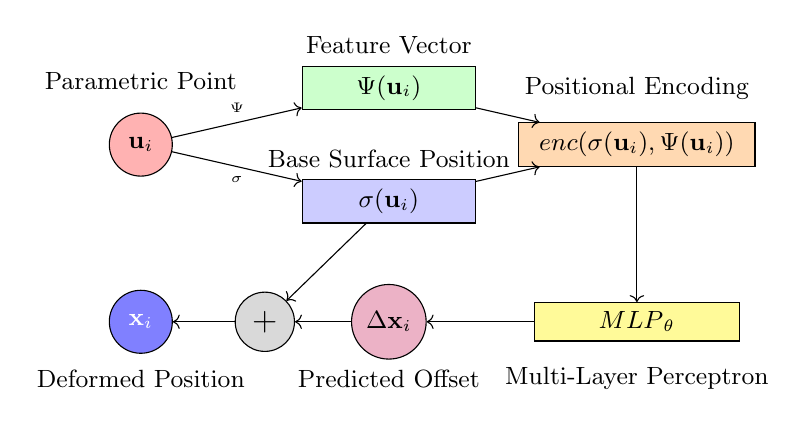
\begin{tikzpicture}[scale=0.9]

    % Sample point u_i
    \node[draw, circle, fill=red!30, minimum size=0.8cm] (u) at (0,0) {\small $\mathbf{u}_i$};
    \node at (0,0.9) {\small Parametric Point};

    % Psi(u)
    \node[draw, rectangle, fill=green!20, minimum width=2.2cm] (psi) at (3.5,0.8) {\small $\Psi(\mathbf{u}_i)$};
    \node at (3.5,1.4) {\small Feature Vector};

    % Sigma(u)
    \node[draw, rectangle, fill=blue!20, minimum width=2.2cm] (sigma) at (3.5,-0.8) {\small $\sigma(\mathbf{u}_i)$};
    \node at (3.5,-0.2) {\small Base Surface Position};

    % Encoding node
    \node[draw, rectangle, fill=orange!30, minimum width=3cm] (enc) at (7,0) {\small $\text{enc}(\sigma(\mathbf{u}_i), \Psi(\mathbf{u}_i))$};
    \node at (7,0.8) {\small Positional Encoding};

    % MLP node
    \node[draw, rectangle, fill=yellow!40, minimum width=2.6cm] (mlp) at (7,-2.5) {\small $\text{MLP}_\theta$};
    \node at (7,-3.3) {\small Multi-Layer Perceptron};

    % Displacement vector
    \node[draw, circle, fill=purple!30, minimum size=0.8cm] (dx) at (3.5,-2.5) {\small $\Delta \mathbf{x}_i$};
    \node at (3.5,-3.3) {\small Predicted Offset};

    % Plus node for summing sigma(ui) and delta_x (smaller + symbol)
    \node[draw, circle, fill=gray!30, minimum size=0.6cm] (plus) at (1.75,-2.5) {\large $+$};

    % Final position
    \node[draw, circle, fill=blue!50, text=white, minimum size=0.8cm] (x) at (0,-2.5) {\small $\mathbf{x}_i$};
    \node at (0,-3.3) {\small Deformed Position};

    % Arrows
    \draw[->] (u) -- (psi) node[midway, above] {\tiny $\Psi$};
    \draw[->] (u) -- (sigma) node[midway, below] {\tiny $\sigma$};
    \draw[->] (sigma) -- (enc);
    \draw[->] (psi) -- (enc);
    \draw[->] (enc) -- (mlp);
    \draw[->] (mlp) -- (dx);
    \draw[->] (sigma) -- (plus);
    \draw[->] (dx) -- (plus);
    \draw[->] (plus) -- (x);

  \end{tikzpicture}
  \end{adjustbox}
  \caption{Neural displacement pipeline for a sampled point $\mathbf{u}_i$. The point is mapped to a corresponding feature vector $\Psi(\mathbf{u}_i)$ and a base surface position $\sigma(\mathbf{u}_i)$. These inputs are passed through a positional encoding and a learned MLP to produce a displacement vector $\Delta \mathbf{x}_i$. The final deformed position $\mathbf{x}_i$ is obtained by adding the base position and the predicted offset, shown by the plus symbol.}
  \label{fig:neural_displacement}
\end{figure}






\subsubsection{Constructing Connectivity}

Once all displaced vertex positions for a patch are computed, the method constructs mesh connectivity locally for each patch. 
The $k \times k$ grid of vertices is triangulated using a regular pattern, similar to the way elevation data is converted into triangles in height-field rendering. 
Typically, this involves connecting each $2 \times 2$ block of adjacent vertices into two triangles. 
Since each patch is handled independently, this process creates a structured local mesh per patch. 
The final surface mesh is obtained by concatenating the displaced patches, whose boundaries align due to the consistent sampling grid and the result is a semi-regular global mesh. 
This structure strikes a balance between the flexibility of unstructured meshes and the computational efficiency of regular grids, enabling both detailed surface modeling and efficient downstream processing (e.g., rendering or optimization). 
To further improve surface reconstruction quality during mesh extraction, Sivaram and colleagues introduce a jittering strategy that enhances sampling within each patch. 
Rather than relying solely on uniform grid samples, their method perturbs each sample slightly to better capture local surface variations. 
Specifically, given the regular grid sample points
\[\hat{u} = \langle \frac{k-1}{i}, \frac{k-1}{j} \rangle \quad \text{for } 0 \leq i,j \leq k-1,\]
each sample position is randomly offset during optimization by sampling from a disk centered at the origin: 
\[u \sim \hat{u} + D(\omega),\]
where \( D(\omega) \) denotes a uniform distribution over a disk of radius \( \omega \). 
This jittering, applied during optimization, acts as a regularizer that enhances gradient flow and helps capture fine geometric details. 
To avoid artifacts such as triangle fold-overs, the jitter is bounded to a disk of radius less than \( \frac{0.5}{k-1} \), and boundary samples remain unperturbed (\( \omega = 0 \)). 
Additionally, to preserve patch boundaries and maintain alignment between adjacent patches, the jitter amount is set to zero for all boundary samples (\( \omega = 0 \)). 
This randomized sampling approach acts as a regularization mechanism, providing richer gradient signals during optimization and encouraging the neural geometry field to more accurately reconstruct the underlying surface. 
This effect is especially beneficial in regions where vertex density is low (i.e., with fewer or larger patches), allowing the model to capture finer details. 
\begin{figure}[ht]
  \centering
  \begin{adjustbox}{center}
  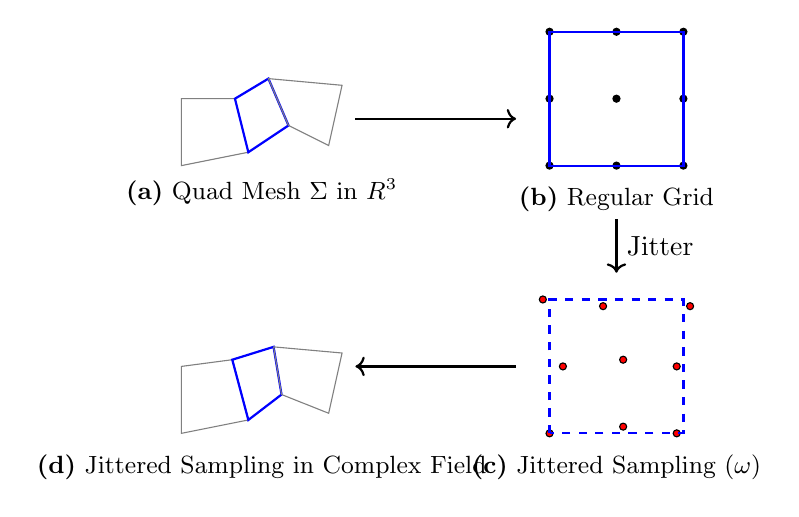
\begin{tikzpicture}[scale=0.85]

    % === (a) Irregular Triangle Mesh ===
    \begin{scope}
      \coordinate (A) at (0,0);
      \coordinate (B) at (1,0.2);
      \coordinate (C) at (0.8,1);
      \coordinate (D) at (0,1);
      \coordinate (E) at (1.6,0.6);
      \coordinate (F) at (1.3,1.3);
      \coordinate (G) at (2.2,0.3);
      \coordinate (H) at (2.4,1.2);

      \draw[gray] (A) -- (B) -- (C) -- (D) -- cycle;
      \draw[blue, thick] (B) -- (E) -- (F) -- (C) -- cycle; % highlighted patch
      \draw[gray] (E) -- (G) -- (H) -- (F) -- cycle;

      \node at (1.2, -0.4) {\small \textbf{(a)} Quad Mesh $\Sigma$ in $\mathbb{R}^3$};
    \end{scope}

    % Arrow
    \draw[->, thick] (2.6,0.7) -- (5.0,0.7) node[midway, above] {};

    % === (b) Regular Grid ===
    \begin{scope}[xshift=5.5cm]
      \foreach \x in {0,1,2} {
        \foreach \y in {0,1,2} {
          \filldraw[black] (\x, \y) circle (1.5pt);
        }
      }

      \draw[blue, thick] (0,0) rectangle (2,2);
      \node at (1,-0.5) {\small \textbf{(b)} Regular Grid};
    \end{scope}

    % Arrow
    \draw[->, thick] (6.5,-0.8) -- (6.5,-1.6) node[midway, right] {Jitter};

    % === (c) Jittered Grid ===
    \begin{scope}[xshift=5.5cm, yshift=-4.0cm]
      \foreach \x/\y in {
        0.0/0.0, 1.1/0.1, 1.9/0.0, 0.2/1.0,
        2.1/1.9, 1.1/1.1, 1.9/1.0, -0.1/2.0,
        0.8/1.9
      } {
        \filldraw[red, draw=black] (\x, \y) circle (1.5pt);
      }

      \draw[blue, thick, dashed] (0,0) rectangle (2,2);
      \node at (1,-0.5) {\small \textbf{(c)} Jittered Sampling ($\omega$)};
    \end{scope}

    % Arrow
    \draw[->, thick] (5.0,-3) -- (2.6,-3) node[midway, above] {};

    % === (d) Irregular Field + Jittered Points ===
    \begin{scope}[yshift=-4.0cm]
      
  \coordinate (A) at (0,0);
  \coordinate (B) at (1.000,0.200); %(1,0.2.0)
  \coordinate (C) at (0.760,1.100); %(0.8,1.0)
  \coordinate (D) at (0,1);
  \coordinate (E) at (1.496,0.580); %(1.6,0.6)
  \coordinate (F) at (1.377,1.292); %(1.3,1.3)
  \coordinate (G) at (2.2,0.3);
  \coordinate (H) at (2.4,1.2);

  \draw[gray] (A) -- (B) -- (C) -- (D) -- cycle;
  \draw[blue, thick] (B) -- (E) -- (F) -- (C) -- cycle; % highlighted patch
  \draw[gray] (E) -- (G) -- (H) -- (F) -- cycle;


  % === Jittered Points Mapped from (c) ===
  %\filldraw[red, draw=black] (1.000,0.200) circle (1.5pt); % (0.0, 0.0)
  %\filldraw[red, draw=black] (1.307,0.385) circle (1.5pt); % (1.1, 0.1)
  %\filldraw[red, draw=black] (1.496,0.580) circle (1.5pt); % (1.9, 0.0)
  %\filldraw[red, draw=black] (0.905,0.700) circle (1.5pt); % (0.2, 1.0)
  %\filldraw[red, draw=black] (1.377,1.292) circle (1.5pt); % (2.1, 1.9)
  %\filldraw[red, draw=black] (1.222,0.885) circle (1.5pt); % (1.1, 1.1)
  %\filldraw[red, draw=black] (1.450,0.880) circle (1.5pt); % (1.9, 1.0)
  %\filldraw[red, draw=black] (0.760,1.100) circle (1.5pt); % (-0.1, 2.0)
  %\filldraw[red, draw=black] (1.091,1.080) circle (1.5pt); % (0.8, 1.9)

  \node at (1.2, -0.5) {\small \textbf{(d)} Jittered Sampling in Complex Field};
\end{scope}


  \end{tikzpicture}
  \end{adjustbox}
  \caption{Progression from an irregular triangle mesh (a) to a regular sampling grid (b), jittered sampling within grid cells (c), and finally applying jittered sampling within a more complex field (d).}
  \label{fig:progression_sampling}
\end{figure}
